%%%%%%%%%%%%%%%%%%%%%%%%%%%%%%%%%%%%%%%%%%%%%%%%%%%%%%%%%%%%%%%%%%%%%%%%%%%%%%%%%%%%%%%%%%%%%
%\chapter{PROBLEM STATEMENT} -- not always required the chapter name as problem statement.	%
% chapter problem statement - in this chapter the problem of the thesis are desribed.				%
%%%%%%%%%%%%%%%%%%%%%%%%%%%%%%%%%%%%%%%%%%%%%%%%%%%%%%%%%%%%%%%%%%%%%%%%%%%%%%%%%%%%%%%%%%%%%
\chapter{OBJECT LOCATION MODEL} 

\section{Probabilistic Modelling}
\label{sec:probability modelling}

Can machines learn from experience? Machine learning as a science has been trying to find a answer to the question from its inception. Machine learning is building knowledge from the data. One approach of building knowledge from data can be to learn the process which generated the data we have observed by creating a model of the process.
\textbf{Probabilistic Modelling} gives us a framework in which we can create such a model, based on our assumptions of the process. The model is basically expressing the assumptions in a mathematical form. The assumptions are the number of variables in the model, the relation between these variables, changes in which variables affects which other variables. This model is then used to generate a problem specific algorithm which can be used to solve the machine learning problem in hand. 

\subsection*{Steps required in Probabilistic Modelling}
\label{sub:steps}
\begin{enumerate}
	\item \textbf{Gather data} to be used for training and evaluation.
    \item \textbf{Gather knowledge} required for model building.
    \item \textbf{Visualise} the data to understand it. This is useful also for gathering knowledge. After visualization the insight gained can be used for assumptions in model building.
    \item \textbf{Construct a model} based on the knowledge of the problem statement available and data visualization. 
    \item \textbf{Perform inference} using both the data and the constructed model. The variables of the model are tuned based on the data available. Predictions can be made to find out the knowledge gained by the model.
    \item \textbf{Evaluate} the performance of the model based on evaluation metric.
    \item \textbf{Diagnose} the model and the assumptions if the evaluation is below some acceptable range
    \item \textbf{Refine the system} by adapting different model structure, inference engine

\end{enumerate}
% subsection steps (end)


\begin{figure}[htp]
\centering
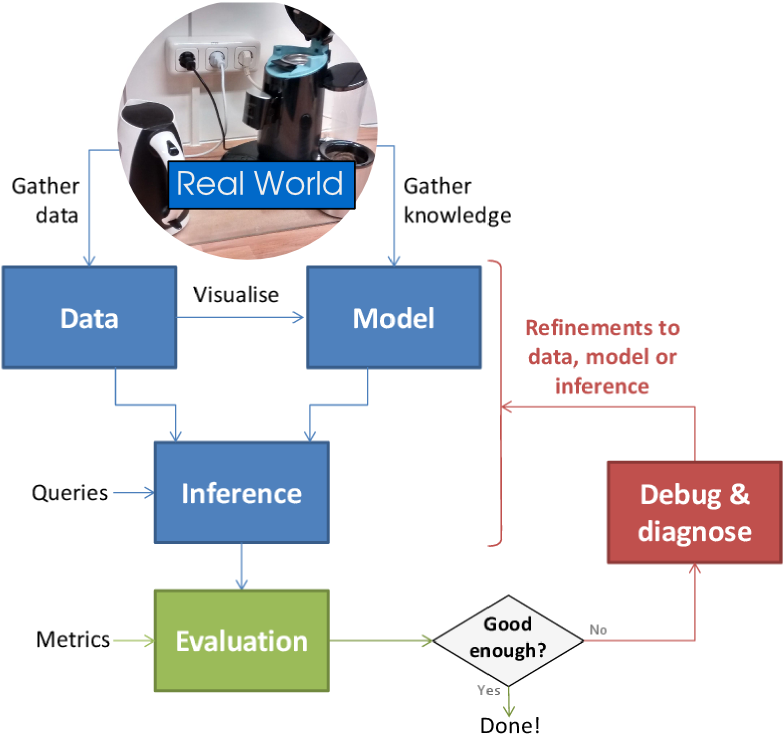
\includegraphics[scale=0.5]{pictures/Lifecycle.png}
\caption{Steps involved in probabilistic modelling  \protect\footnotemark }
\label{}
\end{figure}

\footnotetext{\url{ http://www.mbmlbook.com/LifeCycle.html}}


% section probability modelling (end)
\FloatBarrier
Predicting object location based on the previous seen observations has a lot of challenges. 
\begin{itemize}
	\item  Sparse dataset:-\\
Since the robot is moving around the home and recording the position of objects it has perceived the dataset on which learning has to be performed is sparse. Classical pattern recognition like PCA(eigen vectors)
and variable hidden Markov model will not be able to find pattern in such
sparse dataset. We therefore need a method that can fill in (extrapolate from
observations) large periods of no observability.
    \item Occlusions :- \\
Not only the observations are sparse because of less observations, there is great
sparsity because of occlusions. In a home scenario most of the objects are
always inside containers which cannot be perceived.
    \item Over fitting :- \\
Over fitting is a danger when the number of observation available for learning
is so sparse.
\end{itemize}

As suggested classical machine learning algorithms for finding patterns will not be successful because of the sparseness in the dataset.
The considerations suggest the use of Model based machine learning framework   which allows us to overcome the sparseness in the dataset by creating models and providing some prior information available about object locations in the model.
Furthermore Bayesian non-parametric methods can provide with powerful guards
against over fitting

\section{Problem Formulation}
\label{sec:Problem formulation}

The problem can be formulated as getting an accurate predictive probability density of possible object locations given the previous object locations and the time. Given the corresponding observations of $D_{o_i}$, the probability distribution over the object locations of $o_i$ at time $T$ is governed by the following formula 

    \begin{equation} \label{eq:1}
	    P(l_i | t_i, D_{o_i})
    \end{equation}

   Various temporal information related to periodic patterns can be implied by $T$, to indicate the object's location. Such as specific hours of the day (11:00 pm), a day of the week(Friday), or a month of the year(February). We use the \textbf{temporal state} to represent such information and introduce $r(t)$ to denote temporal state extracted from time $T$,.  Dependency on the type of the temporal state $r(t)$ can be a different function. For example,if $r(t)$ denotes temporal state in terms of hours of the day then $r(t) \in {0,1 ... , 23}$, if $r(t)$ denotes temporal state in terms of day of the week, then $r(t) \in {0,1, .. 6}$ . Without loss of generality, we use $r(t)$ to denote a type of temporal state in the following description, Equation \ref{eq:1} is reformulated as 
    
    \begin{equation}
	    P( l_i | r(t), D_{o_i})
    \end{equation}
    
    Applying Bayes Rule
    
    \begin{equation}\label{eq:3}
	P( l_i | r(t), D_{o_i}) \propto P(r(t) | l_i, D_{o_i})  P(l_i | D_{o_i})
    \end{equation}
    Where:
    \begin{itemize}[label=]
    \item $P(r(t) | l_i, D_{o_i})$ : Temporal context 
    \item $P(l_i | D_{o_i})$ : Spatial context
    \end{itemize}
    
     The spatial context $P(l_i | D_{o_i})$ indicates the location distribution of object $o_i$ given the previous observed location $D_{o_i}$ . The temporal context $P(r(t) | l_i, D_{o_i})$ represents the temporal state distribution of object $o_i$, being observed at location $l_i$ with corresponding $D_{o_i}$
    


\begin{tabular}{cp{8cm}}
    \hline
	Symbol & Meaning\\
	\hline
	O & Set of all Objects\\
	$o_i$ & Single object from the set $O$, $o_i \in O$ \\
	$L$ & Set of all Locations\\
	$l_i$ & Single location from the set $L$. $l_i\in L$\\
    $T$ & Time interval\\
    \hline
	$<o_i,l_i,t_i>$ & Object $o_i$ was located at location $l_i$ at time $t_i$\\
	$D$ & Collection of all objects all observed locations\\
	$D_{o_i}$ & Previous observed locations of $o_i$\\ 
    \hline
     $P(r(t) | l_i, D_{o_i})$ &  Temporal context representing the temporal state distribution of $o_i$ at location $l_i$ given previous observations $D_i$\\
     $P(l_i | D_{o_i})$ & Spatial context representing the location distribution of object $o_i$ given the previous observations $D_{o_i}$\\
    \hline
\end{tabular}
% section Problem formulati (end)

\section{Proposed topics of study in the thesis }
\label{sec:Proposed study}
\begin{itemize}
	\item Temporal Preferences :- $P(r(t) | l_i, D_{o_i})$ \\
	Represents the effects of temporal preferences. It captures the temporal state of a object placement at a location based on the previous observations of the object so far.
	\item Spatial Preferences :- $P(l_i | D_{o_i})$ \\
	Represent the effect of spatial preferences. It captures the location preference of the user where he/she likes to place the object at location $l_i$ based on the previous observations of the object so far.
	\item Temporal-Spatial Co-relation : \\
	\ref{eq:3} combines both the user's temporal context and spatial context corresponding to the co-relations between temporal cyclical information and chronological information.
\end{itemize}
% section  Things to study (end)

\newpage
\section{Proposed Models}

This section mentions the various models which can be used to model the spatio-temporal pattern generation:

\subsection{Gaussian Mixture Model based Naive Bayes Classifier}
\label{sub:GMM}
One of the hypothesis to be examined in the thesis is that the object location has a temporal pattern. The objects locations are decided on the basis of time. For our thesis we will analyse two different type of temporal cyclic patters(daily and weekly).
Since we don't have the location of objects all the time smoothening technique is inevitable to evaluate the probability of a object location at unobserved times.
Mathematically we need a probability distribution to model a user's temporal preference at location $P(r(t) | l_i, D_{o_i})$ . Such distributions should satisfy the following requirements:
\begin{itemize}
	\item Probability distribution centres on one or more temporal state
	\item Probability decreases as the distance to the centre point increases
	\item Each object has a biased probability decreasing speed around the centre
\end{itemize}

Gaussian Mixture Model (GMM) capture these properties.

\subsubsection*{Temporal Cyclic Pattern}
\label{ssub:}
We first formally define $r(t)$ in terms of daily and weekly temporal states. We define $r(t) = {r_d(t), r_w(t)} $ as two indicator function mapping. The timestamp for each type of time where $r_d(t) \in {0,1 .. 23}$ and $r_w(t) \in {0,1 ... 6}$.

So the temporal state can be re-written as :
\begin{equation}
	P(r(t) | l_i, D_{o_i}) = P(r_d(t), r_w(t) | l_i, D_{o_i})
\end{equation}
We will follow independence assumption of daily and weekly patterns.
\begin{equation}
	P(r(t) | l_i, D_{o_i}) = P(r_d(t)| l_i, D_{o_i}) P(r_w(t) | l_i, D_{o_i})
\end{equation}

\begin{figure}[htb] 
\centering 
\def\svgwidth{200pt} 
\input{bayes-model.pdf_tex} 
\caption{Graphical structure of Temporal Cyclic Model. Shaded nodes are observed} 
\end{figure} 
% subsubsection  (end)
% subsection GMM (end)

\FloatBarrier
\subsection*{Dirichlet Process Mixture Model}
\label{sec:dp model}
In this model we assume that the latent discrete locations $l_i$ is not known to us. We would infer this directly from the observations.
Mixture modelling is a well established method for inferring latent discrete variables when we know exactly the clusters involved.
Therefore we use Dirichlet process mixture model that allows us to infer the number of locations, k.

Again, even here to address the problem of filling in large period of missing data, we assume the behaviour is periodic.
% section  (end)
\begin{figure}[htb] 
\centering 
\def\svgwidth{450pt} 
\input{lda-model.pdf_tex} 
\caption{Graphical structure of Latent Dirichlet Model. Shaded nodes are observed, square nodes are fixed values} 
\end{figure} 

\FloatBarrier
\subsection*{Nonparametric Bayesian Model}
For the mixture model mentioned above are defined for a fixed number of categories modelled using dirichlet distribution. Now imagine generalizing the combination of dirichlet over infinitely number of categories. Just as in the Dirichlet distribution we fixed the number of locations to k, the number of locations in Nonparametric Bayesian model is $ \infty $ . The non-parametric, or infinite, models have a number of useful mathematical properties which is useful in determining patterns in sparse dataset.

% section  Proposed Models(end)


\section{Tools for Probability Modelling}
\label{sec:tools}

The separation of the model choices and the inference engine for generating machine algorithms have given rise to a new kind of software frameworks.
In the software framework you need to provide the description of your model and the selection of the inference engine, which internally produces the code for the machine learning algorithm.
Examples of software frameworks that implement the probabilistic modelling philosophy  include CHURCH \cite{goodman_church_2012}, Venture \cite{mansinghka_venture_2014}, PyMC3 \cite{salvatier_probabilistic_2015}, BayesPy \cite{luttinen_bayespy_2014} and Infer.net \cite{minka_2010}.


\textbf{BayesPy} provides tools to do probabilistic modelling. In BayesPy users construct their models, observes data and then runs inference. The inference engine present in BayesPy is variational Bayesian inference.

\textbf{PyMC3} is python module for Bayesian modelling. It provides intuitive model specification syntax for designing the models. The inference is primarily focussed on advanced Markov chain Monto Carlo fitting algorithms.

 
% section tools (end)

\subsection{Limitations }
\label{sub:}

In the thesis we predict the object locations based on previous observations. The basic assumption is that the objects are different types and there are no multiple objects of same type. For example for modelling multiple spoons. The current modelling technique doesn't incorporate modelling for multiple instances of single object.
 
The data collection as explained is a passive process. Basically it means that the robot collects the data when it is doing its daily activity. So if the robot doesn't happen to do any other activity the data collection is stopped.
There are also chances that when the robot is on a particular place the object is occluded always.

If the frequency of the data collection is less than the movement of the object the model will be limited in making predictions only on the locations it has data. So for the locations which the model has no recordings, predictions will not be made.


% subsection  (end)
